% 对偶空间：对偶映射与转置。

\section{对偶映射}
\label{sec:ls-dual-map}

已知线性映射$T:V\to W$和输出端的一个读取$f\in W^*$，输入$\bm x$经过$T$以后被读成$f(T\bm x)$。先作用、再读取，合起来是输入端的一个读取。由这一复合定义\term{对偶映射}（dual map）$T':W^*\to V^*$：
\begin{equation}
\begin{gathered}
T'f=f\circ T\\
(T'f)(\bm x)=f(T\bm x).
\end{gathered}
\label{eq:ls-dual-map-def}
\end{equation}
$T'$保持线性组合：
\[
 \bigl(T'(\alpha f+\beta g)\bigr)(\bm x)=\alpha f(T\bm x)+\beta g(T\bm x).
\]
对象从$V$走到$W$，读取则从$W^*$传回$V^*$，方向相反；这只是把读取规则搬回输入端，不是对$T$求逆。

复合时次序也随之反转：对$S:W\to U$，
\[
 (S\circ T)'f=f\circ S\circ T=T'(S'f),
\]
即$(S\circ T)'=T'\circ S'$。


图~\ref{fig:v2-dual-pullback}比较先变换再读取与直接在输入端读取的两条路线。两条路线的终点读数相同，因此这里搬回的是读取规则。
\begin{figure}[!htb]
\centering
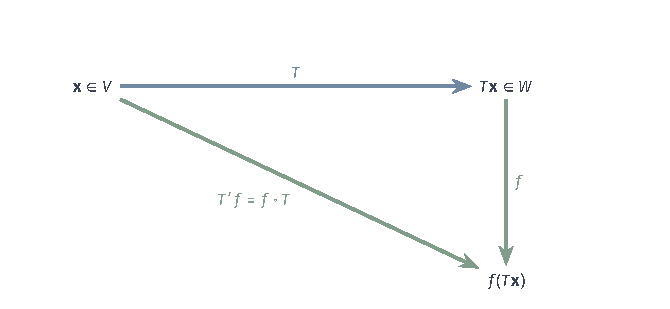
\includegraphics[width=112mm]{figures/02-vectors-matrices-and-multivariate-calculus/01-vectors-and-linear-spaces/tikz/explanation-additions/dual-pullback.pdf}
\caption{对偶映射由复合定义。蓝箭头为对象的线性变换，绿色箭头为标量读取；$f$在输出端读取，$T^{\prime}f$在输入端读取。图中没有从$W$到$V$的逆变换，$T$即使不可逆也能定义$T^{\prime}$。}
\label{fig:v2-dual-pullback}
\end{figure}

\paragraph{对偶映射的矩阵是转置}
设$T$在输入基$\mathcal B=(\bm b_1,\ldots,\bm b_d)$、输出基$\mathcal C=(\bm c_1,\ldots,\bm c_m)$下的矩阵为$\bm A$，即$T\bm b_j=\sum_ka_{k,j}\bm c_k$；两组基的对偶基分别记为$\varphi_1,\ldots,\varphi_d$与$\psi_1,\ldots,\psi_m$。取输出读取$f=\sum_iy_i\psi_i$，它传回输入端以后，在输入基向量上的读数是
\[
 \begin{aligned}
 (T'f)(\bm b_j)&=f(T\bm b_j)
 =\sum_iy_i\,\psi_i\Bigl(\sum_ka_{k,j}\bm c_k\Bigr)\\
 &=\sum_ia_{i,j}y_i=(\bm A^\top\bm y)_j .
 \end{aligned}
\]
第~\ref{sec:ls-dual-space}节说明，读取在对偶基下的坐标就是它在各基向量上的读数，所以$T'f$的坐标为$\bm A^\top\bm y$。也就是说，在对偶基下，对偶映射的矩阵是$\bm A^\top$。

转置的乘积规则$(\bm B\bm A)^\top=\bm A^\top\bm B^\top$正是$(S\circ T)'=T'\circ S'$的坐标记录。下面用一个具体映射核对这一结论。
\begin{example}[把输出的第一个分量读取传回输入端]
\label{ex:ls-dual-map-first-component}
再看$T(x_1,x_2)=(2x_1+x_2,\ 3x_2)$，它在标准基下的矩阵为
\[
 \bm A=\begin{bmatrix}2&1\\0&3\end{bmatrix}.
\]
在输出端读取第一个分量，即$f=\psi_1$，系数$\bm y=(1,0)^\top$。按定义先作用再读取，
\[
 (T'f)(\bm x)=f(T\bm x)=2x_1+x_2,
\]
传回输入端的读取系数为$(2,1)^\top$。按转置计算，
\[
 \bm A^\top(1,0)^\top=(2,1)^\top,
\]
两种算法一致。

这组系数正是$\bm A$的第一行：输出的第一个分量本来就由第一行与输入相乘得到。
\end{example}
一般地，读取输出的第$i$个分量并传回输入端，得到的读取系数就是$\bm A$的第$i$行，所以$T'$的像在坐标下就是行空间。

\paragraph{再证行秩等于列秩}
对偶映射给出定理~\ref{thm:ls-row-rank-column-rank}的另一个证明，它不把矩阵分解为两个因子，而是计算$T'$的核。$T'f=0$意味着$f(T\bm x)=0$对一切$\bm x$成立，即$f$在$\operatorname{im}T$上恒为零。所以$\ker T'$由对全部可达输出读数为零的读取组成，在坐标下就是$\bm A^\top\bm y=\bm0$，即左零空间。

下面计算它的维数。设$r=\operatorname{rank}T$，取$\operatorname{im}T$的基$\bm c_1,\ldots,\bm c_r$并扩充为$W$的基$\bm c_1,\ldots,\bm c_m$，对偶基为$\psi_1,\ldots,\psi_m$。读取$f=\sum_iy_i\psi_i$在$\operatorname{im}T$上恒为零，当且仅当它在$\bm c_1,\ldots,\bm c_r$上都读到零，即$y_1=\cdots=y_r=0$。所以
\[
 \ker T'=\operatorname{span}\{\psi_{r+1},\ldots,\psi_m\},
\]
维数为$m-r$。

对$T':W^*\to V^*$用秩零度定理，
\[
 \operatorname{rank}T'=\dim W^*-\dim\ker T'=m-(m-r)=r .
\]
$T'$的矩阵是$\bm A^\top$，于是$\operatorname{rank}\bm A^\top=\operatorname{rank}\bm A$。

读取规则至此有了自己的空间、坐标和传递规律。读取的大小，即输入有界时读数最大能有多大，需要先给输入规定范数，由下一节的对偶范数回答。有了内积，读取已经可以写成与固定向量的内积（第~\ref{sec:ls-riesz-representation}节），对偶映射也就随之变成第~\ref{sec:ls-adjoints}节的伴随。
